\documentclass[crop,tikz]{standalone}
\usetikzlibrary{backgrounds}
\colorlet{blue}{cyan}
\tikzset{ inverted/.style={every path/.style={draw=white,text=white}, background rectangle/.style={fill}, show background rectangle }}

\tikzset{>=latex}
\usetikzlibrary{calc}

\begin{document}
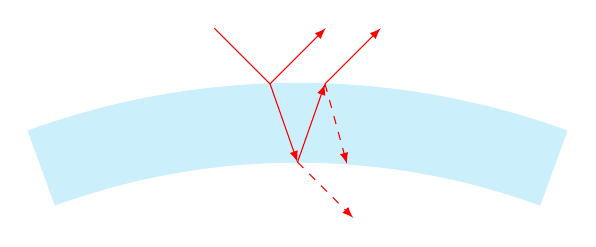
\begin{tikzpicture}
  \draw[fill,cyan!20] (110:10) arc (110:70:10) -- (70:9) arc (70:110:9) -- cycle;
  \coordinate (a) at (92:10);
  \coordinate (b) at (90:9);
  \coordinate (c) at (88:10);
  \draw[->,red] (a)+(135:1) -- (a) -- ($(a)+(45:1)$);
  \draw[->,red] (a) -- (b);
  \draw[->,red] (b) -- (c);
  \draw[->,red] (c) -- ($(c)+(45:1)$);
  \draw[->,red,dashed] (b) -- ($(b)+(-45:1)$);
  \draw[->,red,dashed] (c) -- (86:9);
\end{tikzpicture}
\end{document}
